%!TEX TS-program = xelatex
\documentclass[10pt,oneside]{article}

\usepackage[english]{babel}

\usepackage{amsmath,amssymb,amsfonts}
\usepackage[utf8]{inputenc}
\usepackage[T1]{fontenc}
\usepackage{stix}
\usepackage[scaled]{helvet}
\usepackage[scaled]{inconsolata}

\usepackage{lastpage}

\usepackage{setspace}

\usepackage{ccicons}

\usepackage[hang,flushmargin]{footmisc}

\usepackage{geometry}

\setlength{\parindent}{0pt}
\setlength{\parskip}{6pt plus 2pt minus 1pt}

\usepackage{fancyhdr}
\renewcommand{\headrulewidth}{0pt}\providecommand{\tightlist}{%
  \setlength{\itemsep}{0pt}\setlength{\parskip}{0pt}}

\makeatletter
\newcounter{tableno}
\newenvironment{tablenos:no-prefix-table-caption}{
  \caption@ifcompatibility{}{
    \let\oldthetable\thetable
    \let\oldtheHtable\theHtable
    \renewcommand{\thetable}{tableno:\thetableno}
    \renewcommand{\theHtable}{tableno:\thetableno}
    \stepcounter{tableno}
    \captionsetup{labelformat=empty}
  }
}{
  \caption@ifcompatibility{}{
    \captionsetup{labelformat=default}
    \let\thetable\oldthetable
    \let\theHtable\oldtheHtable
    \addtocounter{table}{-1}
  }
}
\makeatother

\usepackage{array}
\newcommand{\PreserveBackslash}[1]{\let\temp=\\#1\let\\=\temp}
\let\PBS=\PreserveBackslash

\usepackage[breaklinks=true]{hyperref}
\hypersetup{colorlinks,%
citecolor=blue,%
filecolor=blue,%
linkcolor=blue,%
urlcolor=blue}
\usepackage{url}

\usepackage{caption}
\setcounter{secnumdepth}{0}
\usepackage{cleveref}

\usepackage{graphicx}
\makeatletter
\def\maxwidth{\ifdim\Gin@nat@width>\linewidth\linewidth
\else\Gin@nat@width\fi}
\makeatother
\let\Oldincludegraphics\includegraphics
\renewcommand{\includegraphics}[1]{\Oldincludegraphics[width=\maxwidth]{#1}}

\usepackage{longtable}
\usepackage{booktabs}

\usepackage{color}
\usepackage{fancyvrb}
\newcommand{\VerbBar}{|}
\newcommand{\VERB}{\Verb[commandchars=\\\{\}]}
\DefineVerbatimEnvironment{Highlighting}{Verbatim}{commandchars=\\\{\}}
% Add ',fontsize=\small' for more characters per line
\usepackage{framed}
\definecolor{shadecolor}{RGB}{248,248,248}
\newenvironment{Shaded}{\begin{snugshade}}{\end{snugshade}}
\newcommand{\KeywordTok}[1]{\textcolor[rgb]{0.13,0.29,0.53}{\textbf{#1}}}
\newcommand{\DataTypeTok}[1]{\textcolor[rgb]{0.13,0.29,0.53}{#1}}
\newcommand{\DecValTok}[1]{\textcolor[rgb]{0.00,0.00,0.81}{#1}}
\newcommand{\BaseNTok}[1]{\textcolor[rgb]{0.00,0.00,0.81}{#1}}
\newcommand{\FloatTok}[1]{\textcolor[rgb]{0.00,0.00,0.81}{#1}}
\newcommand{\ConstantTok}[1]{\textcolor[rgb]{0.00,0.00,0.00}{#1}}
\newcommand{\CharTok}[1]{\textcolor[rgb]{0.31,0.60,0.02}{#1}}
\newcommand{\SpecialCharTok}[1]{\textcolor[rgb]{0.00,0.00,0.00}{#1}}
\newcommand{\StringTok}[1]{\textcolor[rgb]{0.31,0.60,0.02}{#1}}
\newcommand{\VerbatimStringTok}[1]{\textcolor[rgb]{0.31,0.60,0.02}{#1}}
\newcommand{\SpecialStringTok}[1]{\textcolor[rgb]{0.31,0.60,0.02}{#1}}
\newcommand{\ImportTok}[1]{#1}
\newcommand{\CommentTok}[1]{\textcolor[rgb]{0.56,0.35,0.01}{\textit{#1}}}
\newcommand{\DocumentationTok}[1]{\textcolor[rgb]{0.56,0.35,0.01}{\textbf{\textit{#1}}}}
\newcommand{\AnnotationTok}[1]{\textcolor[rgb]{0.56,0.35,0.01}{\textbf{\textit{#1}}}}
\newcommand{\CommentVarTok}[1]{\textcolor[rgb]{0.56,0.35,0.01}{\textbf{\textit{#1}}}}
\newcommand{\OtherTok}[1]{\textcolor[rgb]{0.56,0.35,0.01}{#1}}
\newcommand{\FunctionTok}[1]{\textcolor[rgb]{0.00,0.00,0.00}{#1}}
\newcommand{\VariableTok}[1]{\textcolor[rgb]{0.00,0.00,0.00}{#1}}
\newcommand{\ControlFlowTok}[1]{\textcolor[rgb]{0.13,0.29,0.53}{\textbf{#1}}}
\newcommand{\OperatorTok}[1]{\textcolor[rgb]{0.81,0.36,0.00}{\textbf{#1}}}
\newcommand{\BuiltInTok}[1]{#1}
\newcommand{\ExtensionTok}[1]{#1}
\newcommand{\PreprocessorTok}[1]{\textcolor[rgb]{0.56,0.35,0.01}{\textit{#1}}}
\newcommand{\AttributeTok}[1]{\textcolor[rgb]{0.77,0.63,0.00}{#1}}
\newcommand{\RegionMarkerTok}[1]{#1}
\newcommand{\InformationTok}[1]{\textcolor[rgb]{0.56,0.35,0.01}{\textbf{\textit{#1}}}}
\newcommand{\WarningTok}[1]{\textcolor[rgb]{0.56,0.35,0.01}{\textbf{\textit{#1}}}}
\newcommand{\AlertTok}[1]{\textcolor[rgb]{0.94,0.16,0.16}{#1}}
\newcommand{\ErrorTok}[1]{\textcolor[rgb]{0.64,0.00,0.00}{\textbf{#1}}}
\newcommand{\NormalTok}[1]{#1}

\newlength{\cslhangindent}
\setlength{\cslhangindent}{1.5em}
\newlength{\csllabelwidth}
\setlength{\csllabelwidth}{3em}
\newenvironment{CSLReferences}[3] % #1 hanging-ident, #2 entry spacing
 {% don't indent paragraphs
  \setlength{\parindent}{0pt}
  % turn on hanging indent if param 1 is 1
  \ifodd #1 \everypar{\setlength{\hangindent}{\cslhangindent}}\ignorespaces\fi
  % set entry spacing
  \ifnum #2 > 0
  \setlength{\parskip}{#2\baselineskip}
  \fi
 }%
 {}
\usepackage{calc} % for \widthof, \maxof
\newcommand{\CSLBlock}[1]{#1\hfill\break}
\newcommand{\CSLLeftMargin}[1]{\parbox[t]{\maxof{\widthof{#1}}{\csllabelwidth}}{#1}}
\newcommand{\CSLRightInline}[1]{\parbox[t]{\linewidth}{#1}}
\newcommand{\CSLIndent}[1]{\hspace{\cslhangindent}#1}\usepackage[table,dvipsnames]{xcolor}

\geometry{includemp,
            letterpaper,
            top=1.2in,
            bottom=2.510cm,
            inner=0.6in,
            outer=0.5in,
            marginparwidth=2in,
            marginparsep=0.5in}

\usepackage[singlelinecheck=off]{caption}
\captionsetup{
  font={small},
  labelfont={bf},
  format=plain,
  labelsep=quad
}
\usepackage{floatrow}
\floatsetup[figure]{margins=hangright,
              facing=no,
              capposition=beside,
              capbesideposition={center,outside},
              floatwidth=\textwidth}
\floatsetup[table]{margins=hangoutside,
             facing=yes,
             capposition=beside,
             capbesideposition={center,outside},
             floatwidth=\textwidth}

\pagestyle{plain}

\setcounter{secnumdepth}{5}

\usepackage{titlesec}

\titleformat{\section}[block]
{\normalfont\large\sffamily}
{\thesection}{.5em}{\titlerule\\[.8ex]\bfseries}

\titleformat{\subsection}[runin]
{\normalfont\fontseries{b}\selectfont\filright\sffamily}
{\thesubsection.}{.5em}{}

\titleformat{\subsubsection}[runin]
{\normalfont\itshape\sffamily}{(\thesubsubsection)}{1em}{}

\fancypagestyle{firstpage}
{
   \fancyhf{}
   \renewcommand{\headrulewidth}{0pt}
   \fancyfoot[R]{\footnotesize\ccby}
   \fancyfoot[L]{\footnotesize\sffamily\today}
}

\fancypagestyle{normal}
{
  \fancyhf{}
  \fancyfoot[R]{\footnotesize\sffamily\thepage\ of \pageref*{LastPage}}
}

\usepackage{tikz}
\begin{document}
\tikz [remember picture, overlay] %
\node [shift={(-0.6in,1.1cm)},scale=0.2,opacity=0.4] at (current page.south east)[anchor=south east]{
\includegraphics{logo}};%
\pagestyle{normal}
\thispagestyle{firstpage}

\newcommand{\colorRule}[3][black]{\textcolor[HTML]{#1}{\rule{#2}{#3}}}

\noindent {\LARGE \textbf{\textsf{Linear Filtering as an imputation
method for Singular Value Decomposition inference of host-virus
associations}}}

\medskip
\begin{flushleft}
{\small
Marie-Andrée\,Ouellet\,\textsuperscript{1}, Gregory\,Albery\,\textsuperscript{2}, Dan\,Becker\,\textsuperscript{3}, Colin
J.\,Carlson\,\textsuperscript{4,5}, Timothée\,Poisot\,\textsuperscript{1,6,*}
\vskip 1em
\textsuperscript{1}\,Département de Sciences Biologiques, Université de
Montréal; \textsuperscript{2}\,Department of Biology, Georgetown
University; \textsuperscript{3}\,Department of Biology, University of
Oklahoma; \textsuperscript{4}\,Center for Global Health Science and
Security, Georgetown University Medical
Center; \textsuperscript{5}\,Department of Microbiology and Immunology,
Georgetown University Medical Center; \textsuperscript{6}\,Québec Centre
for Biodiversity Sciences\\
\textsuperscript{*}\,\,\texttt{timothee.poisot@umontreal.ca}
}
\end{flushleft}

\vskip 2em
\makebox[0pt][l]{\colorRule[CCCCCC]{2.0\textwidth}{0.5pt}}
\vskip 2em
\noindent

\marginpar{\vskip 1em\flushright
{\small{\bfseries Keywords}:\par
viral ecology\\imputation\\singular value decomposition\\ecological
network inference\\}
}


\textbf{Abstract}:\,The current pandemic of SARS-CoV-2 is a stark
reminder that we need a better understanding of the movements of viruses
through novel animal hosts, and ultimately to humans. The task of
predicting which virus can infect which host, and where spillovers are
likely to happen, still remains difficult. Typically, anticipatory
approaches can be limited by numerous difficulties (lack of suitable
data, disagreement between models, etc.), and would therefore benefit
from adding methods allowing imputation and producing results that could
easily be added to ensemble models. In this study, we explore the
potential of using the Singular Value Decomposition (SVD) technique as
an imputation method to predict host-virus interactions.

\vskip 2em
\makebox[0pt][l]{\colorRule[CCCCCC]{2.0\textwidth}{0.5pt}}
\vskip 2em

\textbf{TK} rework this paragraph: need to predict host-virus
associations

The current pandemic of SARS-CoV-2 is a stark reminder that movement of
viruses through novel animal hosts, and ultimately to human through
zoonotic spillovers (Plowright et al. 2017), requires that we understand
the complexity of our biological surroundings. Indeed, the fact that the
majority of emerging infectious diseases are caused by zoonotic
pathogens from wildlife sources (Jones et al. 2008) gives some urgency
to the task of predicting which viruses can be found in which hosts, so
as to provide guidance on where and what species to sample and where
spillovers are likely to happen (Johnson et al. 2020; Albery et al.
2020).

As seen with SARS-CoV and MERS-CoV epidemics, novel human infections by
viruses are representing a serious threat to global public health, and
being able to prevent future viral emergence now appears as a
fundamental tool among our society. Zoonotic dynamics usually involve
three main stages: transmission within the animal reservoir,
cross-species spillover and transmission to human, and finally,
transmission among humans (Lloyd-Smith et al. 2009). In the past
decades, substantial research effort has been put in studying and
predicting dynamics at the animal-human interface, but tracing back the
ultimate origin of novel zoonotic viruses remains a major difficulty
(Becker et al. 2020). Also, the main strategy adopted so far against
infectious diseases consists in taking actions after the emergence by
increasing the health infrastructures and vigilance, as well as
developing vaccines or medical treatments (Han and Drake 2016).

As suggested by Han and Drake (2016), a more efficient approach would be
anticipatory. Yet an anticipatory approach can be limited by lack of
suitable data, and as Becker et al. (2020) highlighted, by disagreement
between models. The task of predicting possible host-virus interactions
would therefore benefit from adding methods that allow imputation, and
can produce results that are easily added to ensemble models. Here, we
explore an approach focusing on the first stage of zoonoses dynamics, by
using the Singular Value Decomposition (SVD) as an imputation method for
identifying unobserved host-virus interactions, acting as potential
intermediate hosts in diseases transmissions.

\textbf{TK} SVD is a way to do link prediction in the absence of
external information, but we can rely on info contained in the network
itself

\textbf{TK} main results: optimal rank, number of new associations, top
10 zoonoses

\hypertarget{dataset}{%
\section{Dataset}\label{dataset}}

\textbf{TK} this actually uses CLOVER now

We apply SVD imputation to the data on wildlife hosts of
beta-coronaviruses collected by Becker et al. (2020). This host-virus
network is composed of 710 mammalian hosts (resolved at the species
level) and 72 viruses (resolved at the genus level). Full data are
available from \texttt{https://github.com/viralemergence/virionette/}.
While the host-virus interaction have been pulled from published
sources, specific attention has been paid to betacoronaviruses, a viral
genus at high risk of spillover, and to their potential bat hosts, a
mammalian order known to be evolutionary involved in the main viruses
zoonotic historical epidemics (Shipley et al. 2019; Ren et al. 2006).
Data on interactions between these groups were augmented by a GenBank
search to retrieve the hosts associated to sequences of
betacoronaviruses. Altogether, this dataset represents a total of 1731
unique interactions, and 49389 host-virus pairs for which no interaction
were reported; these can be true negatives (the virus is unable to
infect the host), or false negatives (the virus can infect the host but
the infection has not been reported). This type of problem lends itself
well to an approach using a recommender system.

\hypertarget{the-model}{%
\section{The model}\label{the-model}}

We ran all analyses in \emph{Julia} 1.5.3 (Bezanson et al. 2017), on the
\emph{Beluga} supercomputer operated by the Calcul Québec consortium.

\hypertarget{low-rank-approximation-with-singular-value-decomposition}{%
\subsection{Low-rank approximation with Singular Value
Decomposition}\label{low-rank-approximation-with-singular-value-decomposition}}

Singular Value Decomposition (SVD; Gene H. Golub and Reinsch 1971;
Forsythe and Moler 1967) is a linear algebra technique used to decompose
a data matrix in a product of three matrices:

\begin{equation}\protect\hypertarget{eq:svd}{}{\mathbf{X} =  \mathbf{U \Sigma V}^T}\label{eq:svd}\end{equation}

Where \(\mathbf{X}\) is a \(m \times n\) data matrix (\(m \ge n\)),
\(\mathbf{U}\) is an unitary \(m \times m\) matrix containing the left
singular vectors, \(\mathbf{V}\) is an unitary \(n \times n\) matrix
containing the right singular vectors and \(\mathbf{\Sigma}\) is a
diagonal matrix containing the singular values ordered in decreasing
order of importance, in regard of the quantity of information that they
present. This process allows data reduction by finding key correlations
among entries and then by approximating the original matrix.

Optimal truncation of the SVD at rank \(r\) (Eckart and Young 1936; G.
H. Golub, Hoffman, and Stewart 1987) of the singular values will allow
data reduction while keeping enough information to obtain a balance
between complexity and accuracy within the model. Truncation at rank
\(r\) was performed by setting values \(\mathbf{\Sigma}_{(r+1)..m}\) to
0 (we note the resulting vector \(^{(r)}\mathbf{\Sigma}\)), and the
resulting low-rank approximation was obtained by

\begin{equation}\protect\hypertarget{eq:lowrank}{}{^{(r)}\mathbf{X} =  \mathbf{U} \, ^{(r)}\mathbf{\Sigma \, V}^T}\label{eq:lowrank}\end{equation}

We illustrate the process on our dataset in fig.~\ref{fig:lowrank}.
Removing signal from the matrix through a low-rank approximation hinges
on the assumption that most data are generated by ``low-rank''
processes, whereas the additional ranks would reflect noise or
idiosyncracies acting in the dataset. Under this assumption, an
imputation method using a low-rank approximation would have a good
performance.

\begin{figure}
\hypertarget{fig:lowrank}{%
\centering
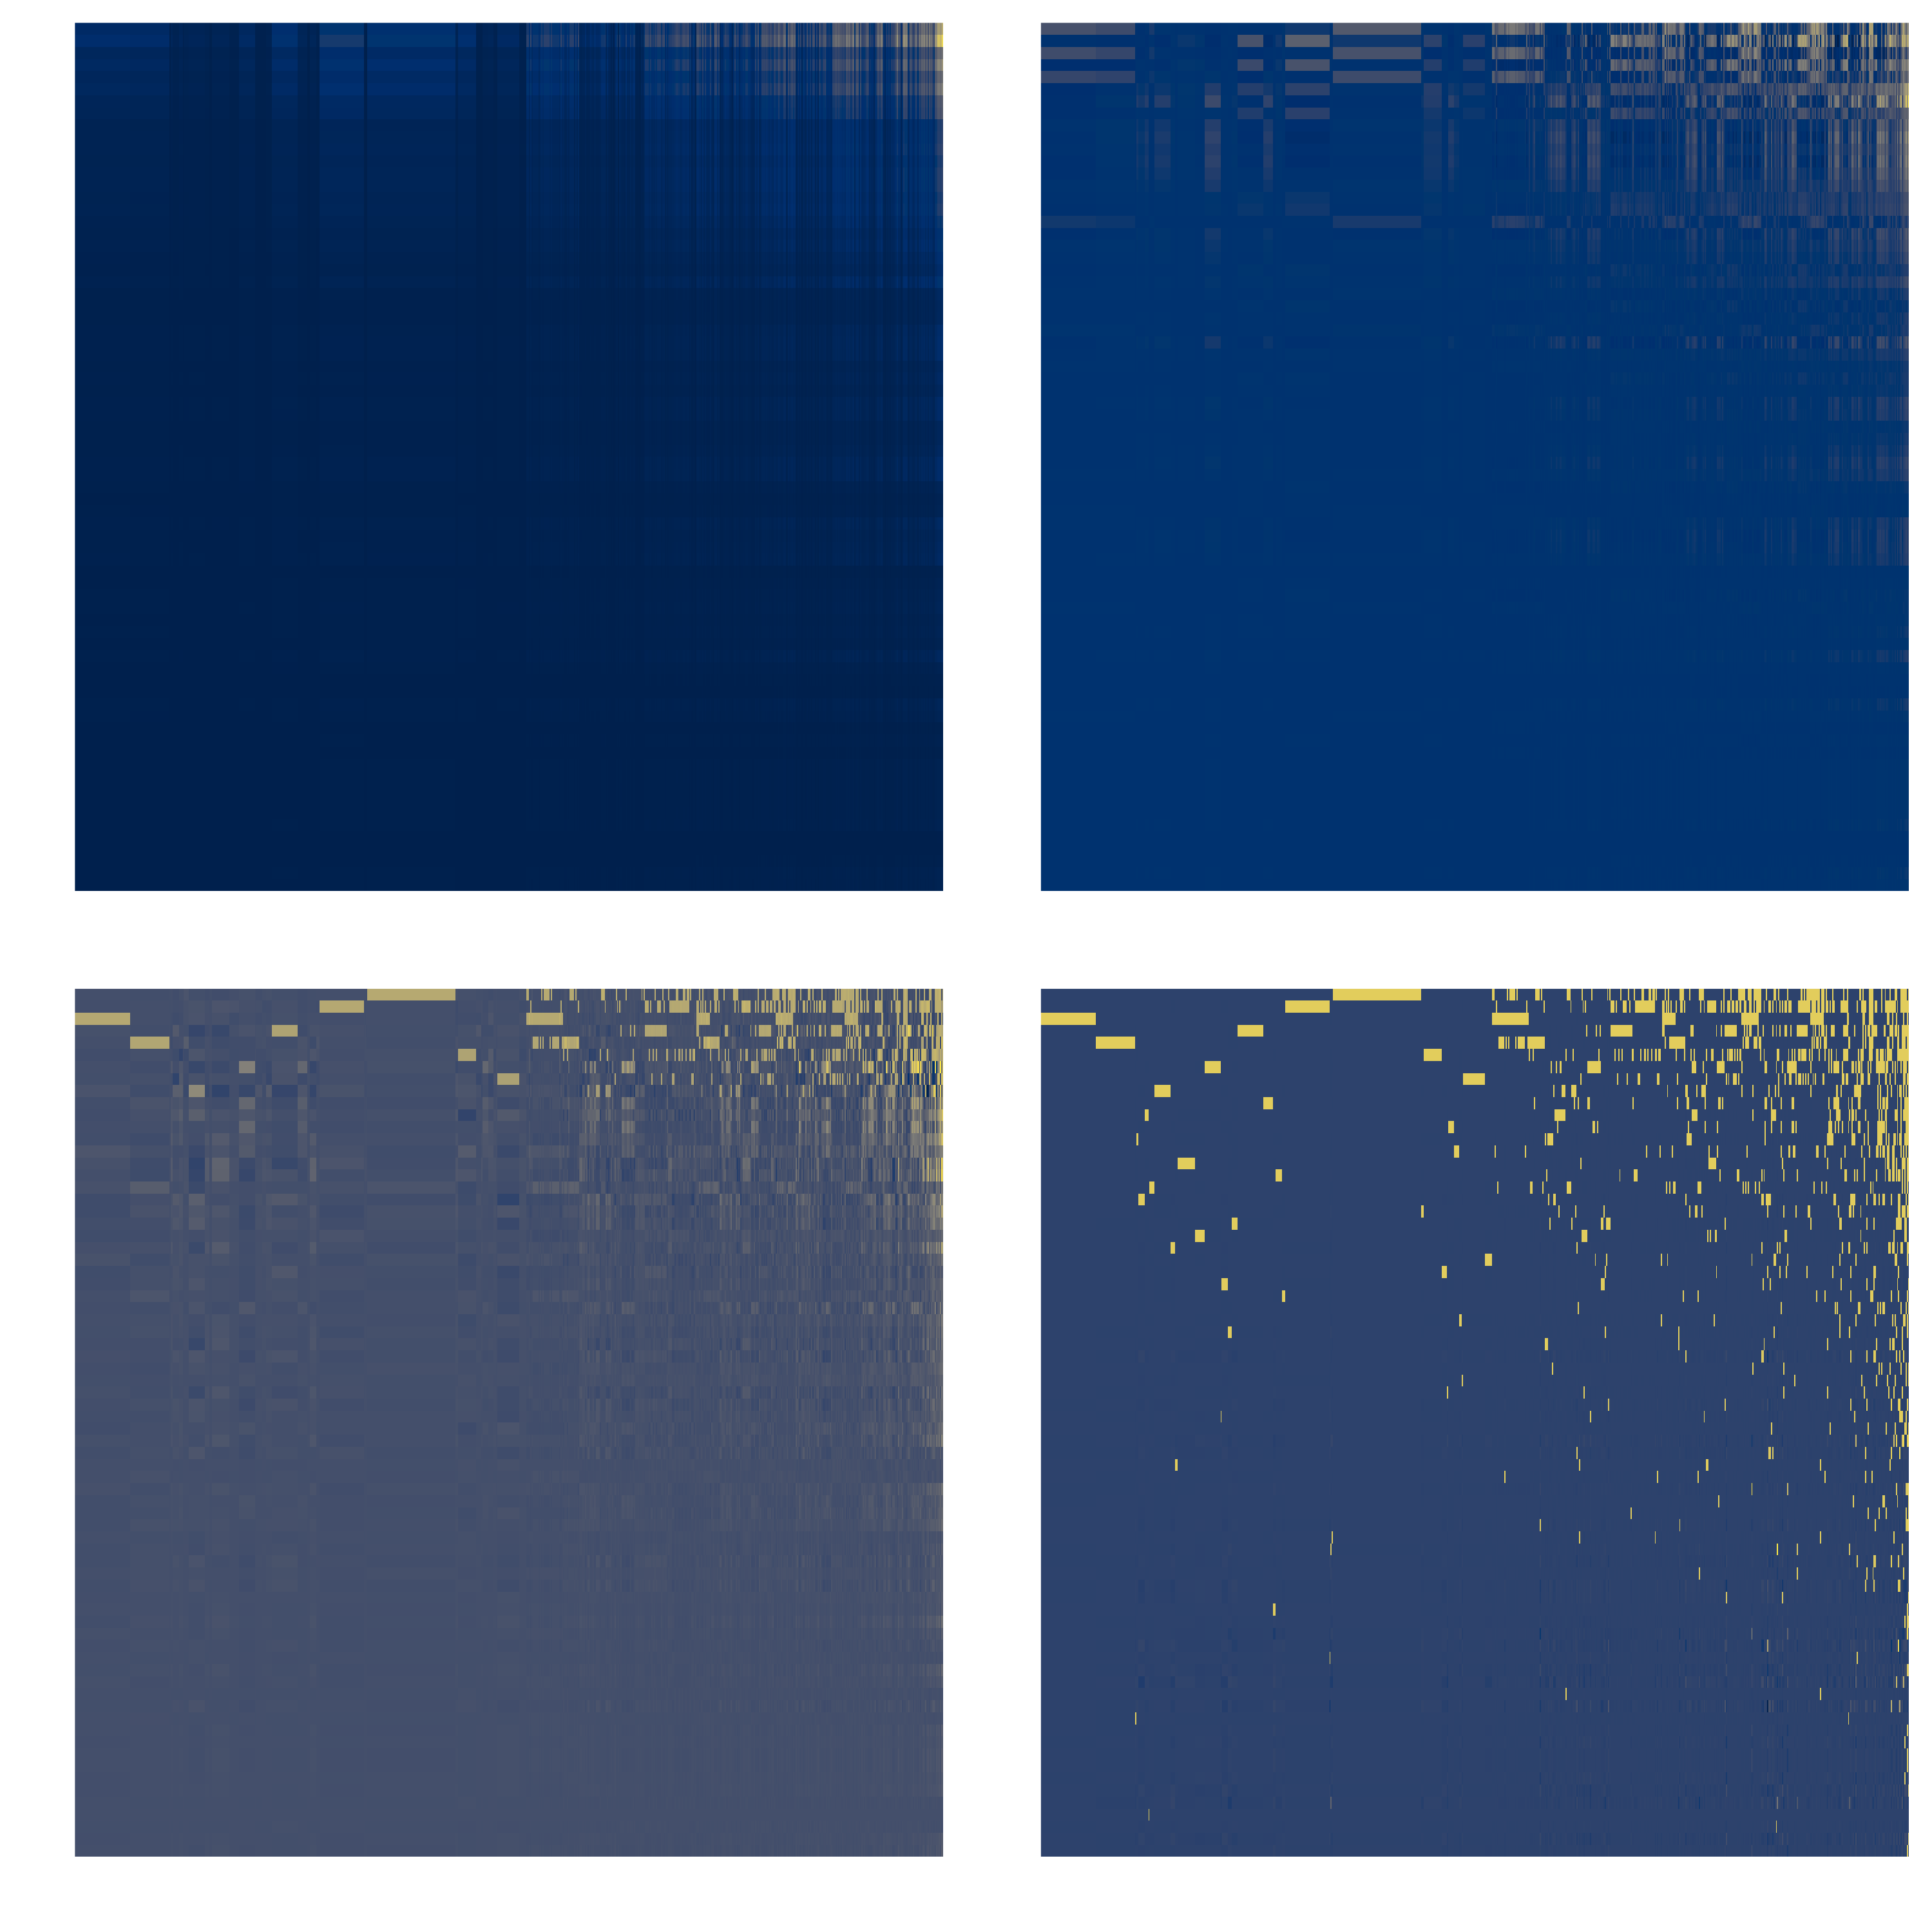
\includegraphics{figures/lowrank_illustration.png}
\caption{Overview of the dataset (yellow means interaction is more
likely, blue means interactions is less likely) at different levels of
approximation. At rank very low rank (top row; from left to right,
\(r=1\) and \(r=3\)) the matrix is mostly capturing the degree of the
different species. At higher ranks (bottom row; from left to right,
\(r=10\) and \(r=60\)), the matrix is capturing increasing differences
in species interactions.}\label{fig:lowrank}
}
\end{figure}

\hypertarget{model-structure}{%
\subsection{Model structure}\label{model-structure}}

For each non-interaction in the dataset, the model assigns an initial
value to it and performs iteratively the SVD at chosen rank, until it
reaches convergence. During this step, the cells in the matrix that are
\emph{not} being imputed are kept at their actual value. We capped the
maximal number of iterations at 50, even though the value of the imputed
cells stopped changing (defined as a step-wise change lower than
\(10\times \epsilon\)) after less than 10 steps in most cases. The
initial value that we first picked for this illustration is the
connectance of the global host-virus interaction dataset, which amounts
to the probability that any pair of organisms are found to interact
(0.03).Yet, this can overestimate the importance of viruses with a
narrow host range, or underestimate the importance of generalist
viruses. For this reason, the assignment of the initial value was then
determined based (Stock et al. 2017) work on linear filtering. This
method provides a convenient way to assign weights to various aspects of
network structure, and has been revealed to provide a good baseline
estimate of how likely it is that a missing interaction actually exists,
based on the structure of the interaction matrix, without the need of
having other side information, such as traits or phylogeny. Considering
our \(m \times n\) data matrix \(\mathbf{X}\), the initial value of a
missing interaction was fixed to the filtered value \(\mathbf{F}_{ij}\)
:

\begin{equation}\protect\hypertarget{eq:linearfiltering}{}{\mathbf{F}_{i,j} =  \mathbf{\alpha_{1}X_{i,j}+\alpha_{2}\frac{1}{m}\sum_{k=1}^m X_{kj} + \alpha_{3}\frac{1}{n}\sum_{l=1}^n X_{il} + \alpha_{4}\frac{1}{mn}\sum_{k=1}^m\sum_{l=1}^n X_{kl} }}\label{eq:linearfiltering}\end{equation}

where \(\sum\limits_{i=1}^4 \alpha_{i} = 1\) and
\(\alpha_{i} \in [0,1]\).

\hypertarget{prediction-scoring}{%
\subsection{Prediction scoring}\label{prediction-scoring}}

Using the linear filter allows to explore different hypotheses as to
which parts of network structure are important for predictive ability.
As we assume that the initial value of 0 in the matrix can be a false
positive, we give it no weight in the model \(\alpha_1 = 0\). \textbf{TK
change from here} We then varied the other parameters on a regular grid
of 304 points, where the values for \(\alpha_4\) (impact of
connectance), \(\alpha_2\) (impact of the number of hosts), and
\(\alpha_3\) (impact of the number of viruses) was varied between 0 and
1. We then applied SVD imputation for each of these parameters
combinations for ranks 1 to 3.

To rank the predictions made by the SVD-imputation, we took the value
for every missing interaction after imputation, and divided it by the
initial value, then substracted one. This gives an evidence score in
\(\mathbb{R}\), which we can transform into a probability in \([0,1]\)
by taking its logistic; therefore, the final probability of an
interaction is defined as

\[
P(x) = \frac{1}{1+e^{-x}}\,,
\]

where \(x\) is the evidence for this interaction under our scoring
system.

\hypertarget{model-tuning-and-thresholding}{%
\subsection{Model tuning and
thresholding}\label{model-tuning-and-thresholding}}

One of the challenges associated with link prediction in this dataset is
that non-interactions are not necessarily true negatives; most are
simply missing data. To reach the best prediction, we need to answer
three related questions. First, what model to assign initial values
performs best? Second, what rank is sufficient to give the most accurate
approximation of the matrix? Finally, what threshold on the interaction
probability should be applied to the results of the best model at the
appropriate rank?

To answer this question, we first ran the LF-SVD imputation on a sample
of 768 positive and 768 supposed negative interactions, at all ranks
from 1 to 20, under the three initial value models above (degree,
hybrid, and connectance). For each of these models, we measured the AUC
of the ROC curve \textbf{REF}. To identify the optimal cutoff in this
curve, we selected the probability score that maximizes Youden's index
of informedness, which works as a ``total evidence'' measure of model
confidence, especially in datasets with severe imbalances in prevalence.

\hypertarget{tbl:modelselection}{}
\begin{longtable}[]{@{}llllllll@{}}
\caption{\label{tbl:modelselection}Summary statistics of the performance
for the top 5 models, ranked according to the area under the ROC curve.
For the sake of completeness, the best Youden's index (at the threshold)
is reported, as well as the rates of false discovery and false
omission.}\tabularnewline
\toprule
& model & rank & threshold & AUC & Youden's index & false discovery &
false omission\tabularnewline
\midrule
\endfirsthead
\toprule
& model & rank & threshold & AUC & Youden's index & false discovery &
false omission\tabularnewline
\midrule
\endhead
1 & connectance & 12 & 0.846 & 0.849 & 0.64 & 0.09 & 0.23\tabularnewline
2 & connectance & 11 & 0.908 & 0.846 & 0.62 & 0.08 & 0.25\tabularnewline
3 & connectance & 17 & 0.929 & 0.844 & 0.62 & 0.08 & 0.24\tabularnewline
4 & connectance & 8 & 0.705 & 0.842 & 0.59 & 0.13 & 0.24\tabularnewline
5 & hybrid & 12 & 0.707 & 0.841 & 0.58 & 0.14 & 0.25\tabularnewline
\bottomrule
\end{longtable}

The resulst of hyper-parameters tuning is presented in
tbl.~\ref{tbl:modelselection}. The best performing model, using network
connectance as an initial value, and a rank 12 approximation of the
matrix, had a positive predictive value of 0.90, and a negative
predictive value of 0.76, for an overall accuracy of 0.82. All things
considered, given that the prevalence in the dataset is very low (only
six out of every thousand species pair do have an interaction), the best
model has strong predictive power. The ROC curve for this model is
presented in fig.~\ref{fig:roc}.

\begin{figure}
\hypertarget{fig:roc}{%
\centering
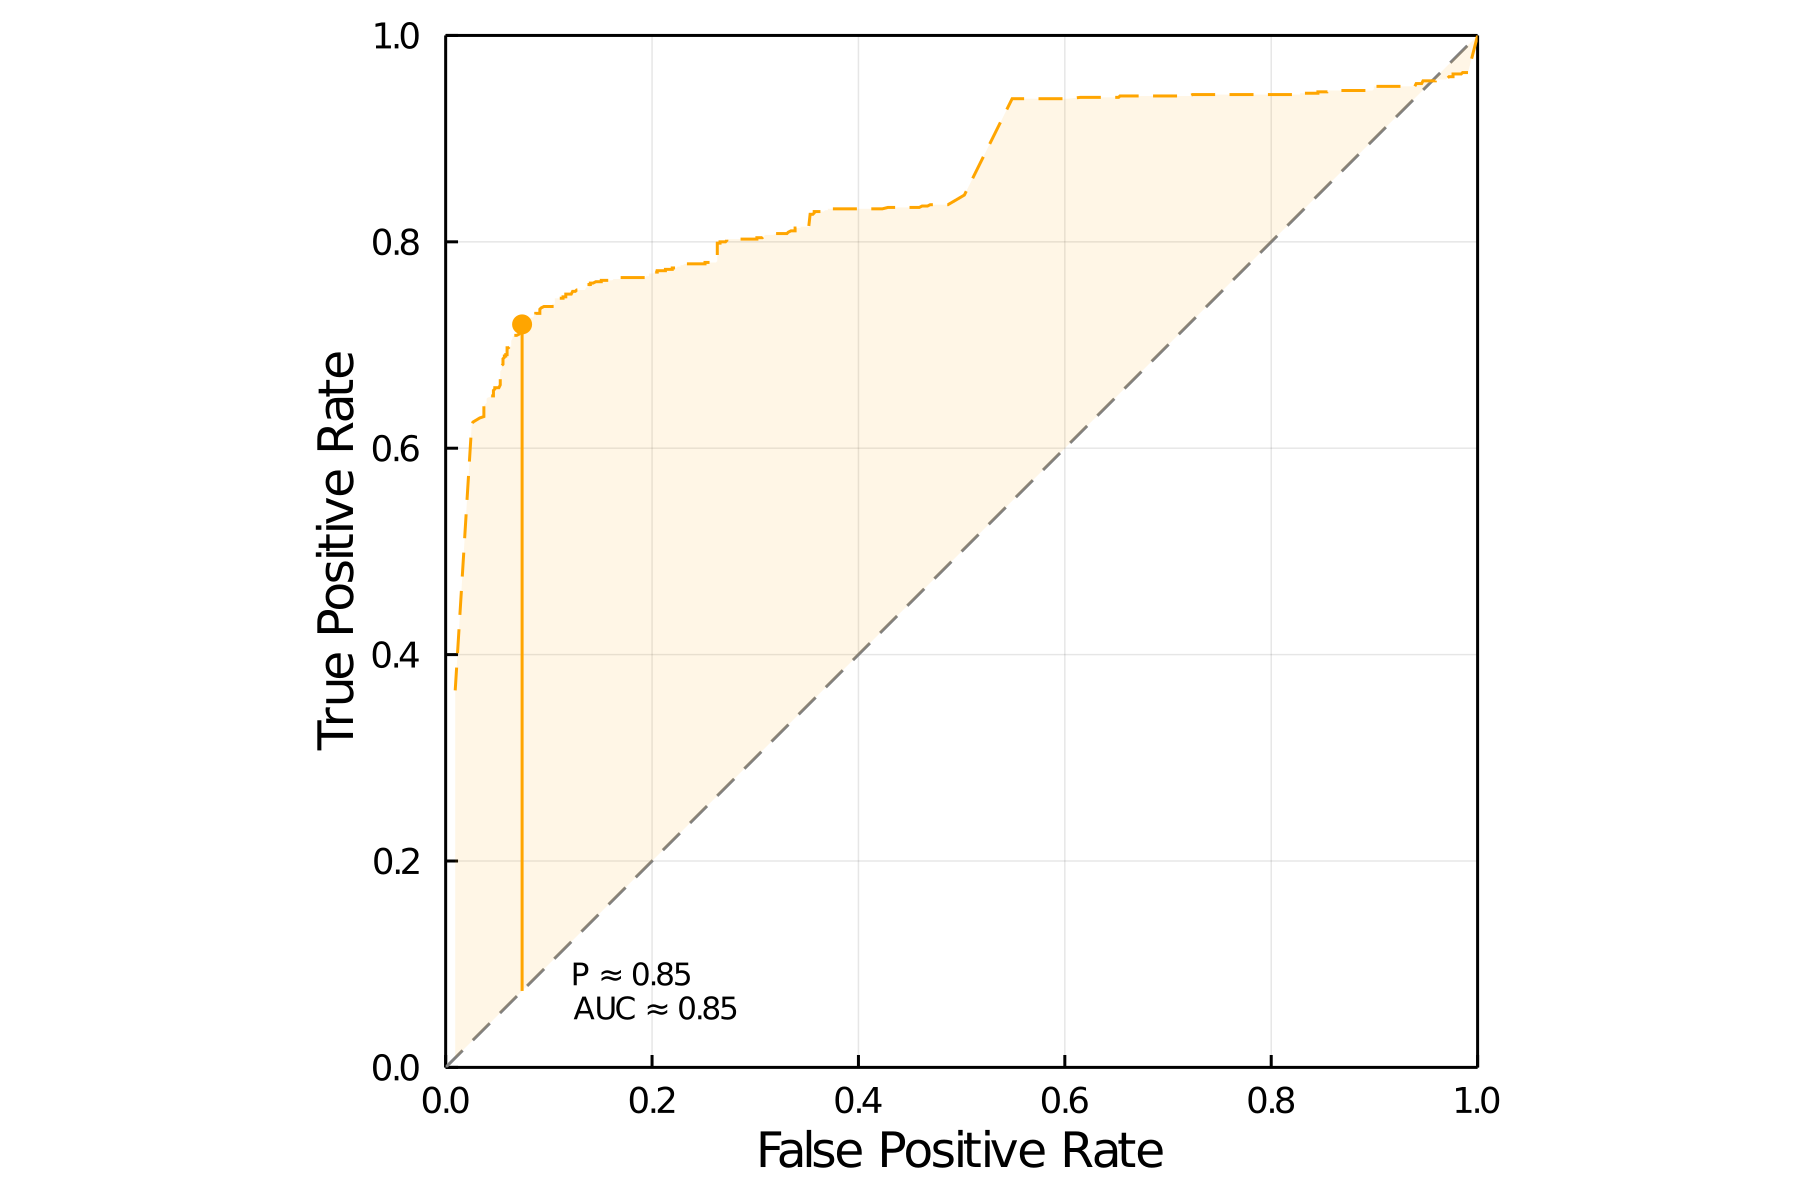
\includegraphics{figures/best-model-roc.png}
\caption{ROC curve for the best model, using network connectance as an
initial value, and a rank 12 approximation. This model was used to run
the prediction of false negatives in the entire dataset.}\label{fig:roc}
}
\end{figure}

\hypertarget{results-and-discussion}{%
\section{Results and Discussion}\label{results-and-discussion}}

First, we report the top 10 likely hosts for betacoronaviruses, using
the connectance of the network as initial values, which are ranked by
their final value post imputation; larger values should indicate that
the interactions are more likely to be possible. We report the novel
hosts (identified post Becker et al. (2020), according to
\texttt{https://www.viralemergence.org/betacov}). These results are
presented in tbl.~\ref{tbl:top10} - the novel hosts are presented in
\textbf{bold}. Using a rank 2 approximation of the dataset, we have 5
novel hosts, and 4 identified as ``suspected'' hosts by the Becker et
al. (2020) ensemble model, currently lacking empirical evidence. This
suggests that rank 2 contains the most information about the processes
generating the data, and can therefore be used to infer other
associations.

\hypertarget{tbl:top10}{}
\begin{longtable}[]{@{}ll@{}}
\caption{\label{tbl:top10}Top 10 likely hosts for betacoronaviruses
using the connectance of the network as initial values}\tabularnewline
\toprule
Rank 1 & Rank 2\tabularnewline
\midrule
\endfirsthead
\toprule
Rank 1 & Rank 2\tabularnewline
\midrule
\endhead
\textbf{Artibeus jamaicensis} & \textbf{Hipposideros
pomona}\tabularnewline
\textbf{Scotophilus kuhlii} & \textbf{Scotophilus kuhlii}\tabularnewline
Molossus rufus & \textbf{Artibeus jamaicensis}\tabularnewline
Sturnira lilium & Carollia brevicauda\tabularnewline
\textbf{Desmodus rotundus} & Chaerephon pumilus\tabularnewline
Glossophaga soricina & Molossus rufus\tabularnewline
Eptesicus fuscus & Glossophaga soricina\tabularnewline
Tadarida brasiliensis & \textbf{Desmodus rotundus}\tabularnewline
Myotis nigricans & Sturnira lilium\tabularnewline
Myotis lucifugus & \textbf{Hipposideros larvatus}\tabularnewline
\bottomrule
\end{longtable}

Based on this information, we have also extracted the 10 highest scoring
interactions across the entire matrix at rank 2 (Table 2). The results
demonstrates that within the entire dataset, including all mammalian
hosts and viruses' genus, 5 out of the 10 highest scoring interactions
are involving bat hosts (presented in \emph{italic}), and 8 out of the
10 interactions are involving the lyssavirus genus. This genus includes
the rabies virus (RABV), and other neurotropic rabies-related viruses
(Warrell and Warrell 2004).

{[}Table 2: Top 10 likely missing interactions across the entire dataset
using the connectance of the network as initial values{]}

\begin{longtable}[]{@{}ll@{}}
\toprule
Hosts species & Viruses genus\tabularnewline
\midrule
\endhead
Sus scrofa & Lyssavirus\tabularnewline
\emph{Hipposideros armiger} & Lyssavirus\tabularnewline
Rattus norvegicus & Lyssavirus\tabularnewline
Myodes glareolus & Lyssavirus\tabularnewline
\emph{Pipistrellus abramus} & Lyssavirus\tabularnewline
Sus scrofa & Orbivirus\tabularnewline
Capra hircus & Alphavirus\tabularnewline
\emph{Rhinolophus sinicus} & Lyssavirus\tabularnewline
\emph{Myotis ricketti} & Lyssavirus\tabularnewline
\emph{Rhinolophus affinis} & Lyssavirus\tabularnewline
\bottomrule
\end{longtable}

Once those results were obtain, further investigations in the form of
literature surveys allowed to identify that the interaction between
\emph{Pipistrellus} abramus\} and lyssaviruses has already been noted by
Hu et al. (2018); Shipley et al. (2019) reported lyssavirus prevalence
in the genus \emph{Pipstrellus}, \emph{Myotis}, and \emph{Rhinolophus}.
Other confirmed hosts of lyssaviruses are \emph{Sus scrofa} (Sato et al.
2004), and \emph{Rattus norvegicus} (Wang, Tang, and Liang 2014).
Surveillance for novel lyssaviruses infections is of great public health
interest, since the rabies virus is fatal in all cases, once the onset
of clinical symptoms has started (Banyard and Fooks 2017). Although it
is recognized that bats are identified as reservoir hosts for
lyssaviruses, the mechanism allowing the maintenance of the virus in
those populations is still poorly understood (Banyard and Fooks 2017),
and these predictions of interactions might serve as guidance in the
monitoring of new infections.

The two non-lyssaviruses associations have been previously reported in
the literature (\emph{Sus scrofa} and orbivirus by Belaganahalli et al.
(2015); \emph{Capra hircus} and the equine encephalomyelitis caused by
an alphavirus as early as Pursell et al. (1972)). This suggests that
Singular Value Decomposition of available data on host-virus
associations can uncover results that have been reported in the primary
literature, but not incorporated in the main databases used in the
field; based on the fact that the majority of the top 10 overall
associations were able to be validated from the literature, we suggest
that interactions that have no empirical evidence could be targets for
additional sampling.

The initial value to be used for the imputation was then assigned
according to the linear filter, as presented in the method section. The
Table 3 presents the number of novel hosts predicted by the model,
according to the coefficients used for the filter and to the rank.

{[}Table 3: Number of novel hosts for betacoronaviruses correctly
predicted by the model using linear filtering for the attribution of
initial values{]}

\begin{longtable}[]{@{}cccccc@{}}
\toprule
Alpha & Rank 1 & Rank 2 & Rank 3 & Rank 4 & Rank 5\tabularnewline
\midrule
\endhead
\textbf{{[}0, 0, 0, 1{]}} & 3 & 3 & 1 & 3 & 4\tabularnewline
\textbf{{[}0, \(\frac{1}{2}\), \(\frac{1}{2}\), 0{]}} & 3 & 3 & 1 & 3 &
3\tabularnewline
\textbf{{[}0, \(\frac{1}{3}\), \(\frac{1}{3}\), \(\frac{1}{3}\){]}} & 3
& 3 & 1 & 4 & 2\tabularnewline
\textbf{{[}0, 1, 0, 0{]}} & 3 & 3 & 1 & 3 & 3\tabularnewline
\textbf{{[}0, 0, 1, 0{]}} & 3 & 3 & 1 & 4 & 3\tabularnewline
\bottomrule
\end{longtable}

From the results presented in Table 3, it is possible to see that when
using linear filtering for the assignment of initial values, the choice
of the \(\alpha\) parameters does not impact the accuracy of the
predictions for the first three rank. The fourth and fifth rank then
showed a variation per \(\alpha\) values. The highest scoring
interactions for every combinations was then examined and the variation
of its value before and after the imputation has been calculated, and
the results obtained are presented in Table 4.

{[}Table 4: Variation of the value pre and post imputation for the
highest scoring interaction at every rank{]}

\begin{longtable}[]{@{}ccccc@{}}
\toprule
Rank 1 & Rank 2 & Rank 3 & Rank 4 & Rank 5\tabularnewline
\midrule
\endhead
0.536 & 0.765 & 0.700 & 0.990 & 1.261\tabularnewline
\bottomrule
\end{longtable}

This variation was not influenced by the \(\alpha\) parameters, but only
by the rank used. The variation calculated increased as the rank got
higher.

Being able to identify intermediate animal hosts for potential zoonotic
pathogens is an important step in the fight against potential threats to
global public health. Using SVD as an imputation method to predict those
interactions has demonstrated its potential to achieve this goal by
correctly identifying the majority of the most likely associations, as
validated by literature surveys, and by suggesting interactions with no
empirical evidence as targets for additional sampling. Host-virus
associations are a challenging imputation problem, because organized
datasets are scarce -- as a result, a lot of missing associations are
reported in the literature, but not available in an easily usable
format. Yet this also presents an opportunity to validate the
performance of recommender systems that is far more interesting than
cross-fold or leave-one-out validation: the existence of these
interactions in the literature can provide validation on data that have
never been used in the modeling process, and therefore provide an
accurate estimate of how frequently existing interactions are
identified. By this measure, that most of the top 10 recommendations on
this dataset were validated through \emph{de novo} sampling (for bat
hosts of betacoronaviruses) or by a literature survey (for the global
dataset) is a strong indication that SVD is able to uncover likely
host-virus pairs.

Future work on the use of SVD for virus host associations will have to
adress the question of the initial value used in the imputation process
in further details. As of now, we relied on the average number of
interactions in the matrix, and on weighted allocations for different
aspects of the network structure, based on Stock et al. (2017) work on
linear filtering. This method can provide a good baseline estimate of
how likely it is that a missing interaction could actually exist (and in
fact was developed for this purpose). For this reason, we are confident
that the performance of the approach can further be improved by
fine-tuning the choice of the initial value used for imputation,
according to the dataset used, or by relying on ensemble models that
would aggregate the output of the best recommenders. Combining an
accurate model for the initial value with the SVD imputation is likely
to generate predicted interactions that are strong candidates for
empirical validation.

\textbf{Acknowledgements:} This research was enabled in part by support
provided by Calcul Québec (www.calculquebec.ca) and Compute Canada
(www.computecanada.ca). TP and CC were funded by IVADO through the rapid
response to COVID special initiative.

\hypertarget{references}{%
\section*{References}\label{references}}
\addcontentsline{toc}{section}{References}

\hypertarget{refs}{}
\begin{CSLReferences}{1}{0}
\leavevmode\hypertarget{ref-Albery2020PreGlo}{}%
Albery, Gregory F., Evan A. Eskew, Noam Ross, and Kevin J. Olival. 2020.
{``Predicting the Global Mammalian Viral Sharing Network Using
Phylogeography.''} \emph{Nature Communications} 11 (1): 2260.
\url{https://doi.org/10.1038/s41467-020-16153-4}.

\leavevmode\hypertarget{ref-Banyard2017ImpNov}{}%
Banyard, Ashley C., and Anthony R. Fooks. 2017. {``The Impact of Novel
Lyssavirus Discovery.''} \emph{Microbiology Australia} 38 (1): 17--21.

\leavevmode\hypertarget{ref-Becker2020PreWil}{}%
Becker, Daniel J., Gregory F. Albery, Anna R. Sjodin, Timothée Poisot,
Tad A. Dallas, Evan A. Eskew, Maxwell J. Farrell, et al. 2020.
{``Predicting Wildlife Hosts of Betacoronaviruses for SARS-CoV-2
Sampling Prioritization.''} \emph{bioRxiv}, May, 2020.05.22.111344.
\url{https://doi.org/10.1101/2020.05.22.111344}.

\leavevmode\hypertarget{ref-Belaganahalli2015GenCha}{}%
Belaganahalli, Manjunatha N., Sushila Maan, Narender S. Maan, Joe
Brownlie, Robert Tesh, Houssam Attoui, and Peter P. C. Mertens. 2015.
{``Genetic Characterization of the Tick-Borne Orbiviruses.''}
\emph{Viruses} 7 (5): 2185--2209.
\url{https://doi.org/10.3390/v7052185}.

\leavevmode\hypertarget{ref-Bezanson2017JulFre}{}%
Bezanson, J., A. Edelman, S. Karpinski, and V. Shah. 2017. {``Julia: A
Fresh Approach to Numerical Computing.''} \emph{SIAM Review} 59 (1):
65--98. \url{https://doi.org/10.1137/141000671}.

\leavevmode\hypertarget{ref-Eckart1936AppOne}{}%
Eckart, Carl, and Gale Young. 1936. {``The Approximation of One Matrix
by Another of Lower Rank.''} \emph{Psychometrika} 1 (3): 211--18.
\url{https://doi.org/10.1007/BF02288367}.

\leavevmode\hypertarget{ref-Forsythe1967ComSol}{}%
Forsythe, George, and Cleve Moler. 1967. \emph{Computer Solution of
Linear Algebraic Systems}. Englewood Cliffs, New Jersey: Prentice Hall.

\leavevmode\hypertarget{ref-Golub1987GenEck}{}%
Golub, G. H., Alan Hoffman, and G. W. Stewart. 1987. {``A Generalization
of the Eckart-Young-Mirsky Matrix Approximation Theorem.''} \emph{Linear
Algebra and Its Applications} 88-89 (April): 317--27.
\url{https://doi.org/10.1016/0024-3795(87)90114-5}.

\leavevmode\hypertarget{ref-Golub1971SinVal}{}%
Golub, Gene H., and Christian Reinsch. 1971. {``Singular Value
Decomposition and Least Squares Solutions.''} In \emph{Linear Algebra},
134--51. Springer.

\leavevmode\hypertarget{ref-Han2016FutDir}{}%
Han, Barbara A., and John M. Drake. 2016. {``Future Directions in
Analytics for Infectious Disease Intelligence: Toward an Integrated
Warning System for Emerging Pathogens.''} \emph{EMBO Reports} 17 (6):
785--89. \url{https://doi.org/10.15252/embr.201642534}.

\leavevmode\hypertarget{ref-Hu2018LysJap}{}%
Hu, Shu-Chia, Chao-Lung Hsu, Ming-Shiuh Lee, Yang-Chang Tu, Jen-Chieh
Chang, Chieh-Hao Wu, Shu-Hwae Lee, et al. 2018. {``Lyssavirus in
Japanese Pipistrelle, Taiwan - Volume 24, Number 4April 2018 - Emerging
Infectious Diseases Journal - CDC.''} \emph{Emerging Infectious
Diseases}. \url{https://doi.org/10.3201/eid2404.171696}.

\leavevmode\hypertarget{ref-Johnson2020GloShi}{}%
Johnson, Christine K., Peta L. Hitchens, Pranav S. Pandit, Julie
Rushmore, Tierra Smiley Evans, Cristin C. W. Young, and Megan M. Doyle.
2020. {``Global Shifts in Mammalian Population Trends Reveal Key
Predictors of Virus Spillover Risk.''} \emph{Proceedings of the Royal
Society B: Biological Sciences} 287 (1924): 20192736.
\url{https://doi.org/10.1098/rspb.2019.2736}.

\leavevmode\hypertarget{ref-Jones2008GloTre}{}%
Jones, Kate E., Nikkita G. Patel, Marc A. Levy, Adam Storeygard, Deborah
Balk, John L. Gittleman, and Peter Daszak. 2008. {``Global Trends in
Emerging Infectious Diseases.''} \emph{Nature} 451 (7181): 990--93.
\url{https://doi.org/10.1038/nature06536}.

\leavevmode\hypertarget{ref-Lloyd-Smith2009EpiDyn}{}%
Lloyd-Smith, James O., Dylan George, Kim M. Pepin, Virginia E. Pitzer,
Juliet R. C. Pulliam, Andrew P. Dobson, Peter J. Hudson, and Bryan T.
Grenfell. 2009. {``Epidemic Dynamics at the Human-Animal Interface.''}
\emph{Science} 326 (5958): 1362--67.
\url{https://doi.org/10.1126/science.1177345}.

\leavevmode\hypertarget{ref-Plowright2017PatZoo}{}%
Plowright, Raina K., Colin R. Parrish, Hamish McCallum, Peter J. Hudson,
Albert I. Ko, Andrea L. Graham, and James O. Lloyd-Smith. 2017.
{``Pathways to Zoonotic Spillover.''} \emph{Nature Reviews Microbiology}
15 (8): 502--10. \url{https://doi.org/10.1038/nrmicro.2017.45}.

\leavevmode\hypertarget{ref-Pursell1972NatOcc}{}%
Pursell, A. R., J. C. Peckham, J. R. Cole, W. C. Stewart, and F. E.
Mitchell. 1972. {``Naturally Occurring and Artificially Induced Eastern
Encephalomyelitis in Pigs.''} \emph{Journal of the American Veterinary
Medical Association} 161 (10): 1143--47.

\leavevmode\hypertarget{ref-Ren2006FulGen}{}%
Ren, Wuze, Wendong Li, Meng Yu, Pei Hao, Yuan Zhang, Peng Zhou, Shuyi
Zhang, et al. 2006. {``Full-Length Genome Sequences of Two SARS-Like
Coronaviruses in Horseshoe Bats and Genetic Variation Analysis.''}
\emph{Journal of General Virology} 87 (11): 3355--59.
\url{https://doi.org/10.1099/vir.0.82220-0}.

\leavevmode\hypertarget{ref-Sato2004GenPhy}{}%
Sato, Go, Takuya Itou, Youko Shoji, Yasuo Miura, Takeshi Mikami, Mikako
Ito, Ichiro Kurane, et al. 2004. {``Genetic and Phylogenetic Analysis of
Glycoprotein of Rabies Virus Isolated from Several Species in Brazil.''}
\emph{Journal of Veterinary Medical Science} 66 (7): 747--53.
\url{https://doi.org/10.1292/jvms.66.747}.

\leavevmode\hypertarget{ref-Shipley2019BatVir}{}%
Shipley, Rebecca, Edward Wright, David Selden, Guanghui Wu, James
Aegerter, Anthony R Fooks, and Ashley C Banyard. 2019. {``Bats and
Viruses: Emergence of Novel Lyssaviruses and Association of Bats with
Viral Zoonoses in the EU.''} \emph{Tropical Medicine and Infectious
Disease} 4 (1). \url{https://doi.org/10.3390/tropicalmed4010031}.

\leavevmode\hypertarget{ref-Stock2017LinFil}{}%
Stock, Michiel, Timothée Poisot, Willem Waegeman, and Bernard De Baets.
2017. {``Linear Filtering Reveals False Negatives in Species Interaction
Data.''} \emph{Scientific Reports} 7 (April): 45908.
\url{https://doi.org/10.1038/srep45908}.

\leavevmode\hypertarget{ref-Wang2014RabRab}{}%
Wang, Lihua, Qing Tang, and Guodong Liang. 2014. {``Rabies and Rabies
Virus in Wildlife in Mainland China, 1990.''} \emph{International
Journal of Infectious Diseases} 25 (August): 122--29.
\url{https://doi.org/10.1016/j.ijid.2014.04.016}.

\leavevmode\hypertarget{ref-Warrell2004RabOth}{}%
Warrell, M. J., and D. A. Warrell. 2004. {``Rabies and Other Lyssavirus
Diseases.''} \emph{The Lancet} 363 (9413): 959--69.
\url{https://doi.org/10.1016/S0140-6736(04)15792-9}.

\end{CSLReferences}

\end{document}
